\usetikzlibrary{decorations.pathreplacing}
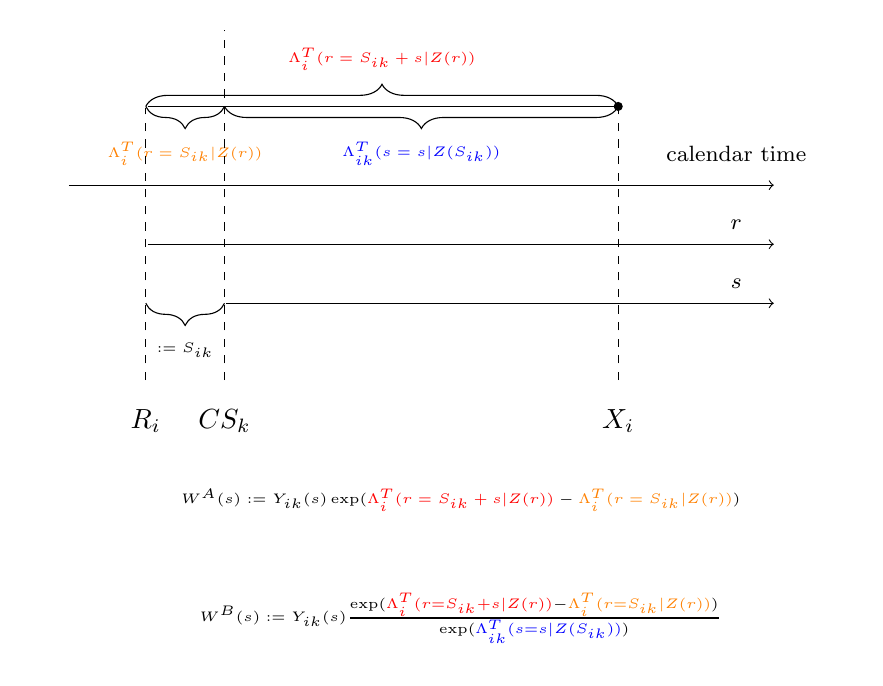
\begin{tikzpicture}
	% Lines are organized from bottom to top
	\path[use as bounding box] (0.5, -6) rectangle (11, 2);
	% Subject 1
	\node[circle, inner sep = 0pt, draw = none] (A) at (2, 1) {};
	\node[circle, inner sep = 0pt, draw , fill, minimum size=.1cm] (B) at (8, 1) {};
	\draw (A) -- (B);
	
	
	% Annotation subject 2
	\draw [decorate,decoration={brace,amplitude=8pt}] (2,1) -- (8,1) node [black,midway,yshift=0.6cm] {\tiny \textcolor{red}{$\Lambda_i^{T}(r = S_{ik} + s | Z(r))$}};
	
	\draw [decorate,decoration={brace,amplitude=8pt,mirror}] (2,1) -- (3,1) node [black,midway,yshift=-0.6cm] {\tiny \textcolor{orange}{$\Lambda_{i}^{T}(r = S_{ik} | Z(r))$}};
	
	\draw [decorate,decoration={brace,amplitude=8pt,mirror}] (3,1) -- (8,1) node [black,midway,yshift=-0.6cm] {\tiny \textcolor{blue}{$\Lambda_{ik}^{T}(s = s | Z(S_{ik}))$}};
	
	%% Vertical lnies
	
	% Vertical line CS_k$.
	\node[circle, inner sep = 0pt, draw = none] (A) at (3, -2.5) {};
	\node[circle, inner sep = 0pt, draw = none] (B) at (3, 2) {};
	\draw[dashed] (A) -- (B);
	
	\node[circle, inner sep = 0pt, draw = none] (A) at (3, -3) {$CS_k$};
	
	
	% Vertical line R_i$.
	\node[circle, inner sep = 0pt, draw = none] (A) at (2, -2.5) {};
	\node[circle, inner sep = 0pt, draw = none] (B) at (2, 1) {};
	\draw[dashed] (A) -- (B);
	
	\node[circle, inner sep = 0pt, draw = none] (A) at (2, -3) {$R_i$};
	
	
	% Accolade for S_{ik}
	\draw [decorate,decoration={brace,amplitude=8pt,mirror}] (2,-1.5) -- (3,-1.5) node [black,midway,yshift=-0.6cm]  {\tiny $:= S_{ik}$};
	
	% Vertical line X_i$.
	\node[circle, inner sep = 0pt, draw = none] (A) at (8, -2.5) {};
	\node[circle, inner sep = 0pt, draw = none] (B) at (8, 1) {};
	\draw[dashed] (A) -- (B);
	
	
	\node[circle, inner sep = 0pt, draw = none] (A) at (8, -3) {$X_i$};
	
	
	%% axes %%
	% Calendar time axis (t)
	\node[circle, inner sep = 0pt, draw = none] (A) at (1, 0) {};
	\node[circle, inner sep = 0pt, draw = none] (B) at (10, 0) {};
	\draw[->] (A) -- (B);
	\node[circle, inner sep = 0pt, draw = none] (A) at (9.5, 0.40)  {\footnotesize calendar time};
	
	% Time since registration (r)
	\node[circle, inner sep = 0pt, draw = none] (A) at (2, -.75) {};
	\node[circle, inner sep = 0pt, draw = none] (B) at (10, -.75) {};
	\draw[->] (A) -- (B);
	\node[circle, inner sep = 0pt, draw = none] (A) at (9.5, -0.5)  {\footnotesize $r$};
	
	% Time since cross-section (s)
	\node[circle, inner sep = 0pt, draw = none] (A) at (3, -1.5) {};
	\node[circle, inner sep = 0pt, draw = none] (B) at (10, -1.5) {};
	\draw[->] (A) -- (B);
	\node[circle, inner sep = 0pt, draw = none] (A) at (9.5, -1.25)  {\footnotesize $s$};
	
	
	%% Weight formulas)
	
	\node[circle, inner sep = 0pt, draw = none] (A) at (6, -4) {\tiny $W^A(s) := Y_{ik}(s)
		\exp(\textcolor{red}{\Lambda_i^{T}(r = S_{ik} + s | Z(r))} - \textcolor{orange}{\Lambda_i^{T}(r = S_{ik} | Z(r))})$}
	;
	
	\node[circle, inner sep = 0pt, draw = none] (A) at (6, -5.5) {\tiny $W^B(s) := Y_{ik}(s) \frac{
			\exp(\textcolor{red}{\Lambda_i^{T}(r = S_{ik} + s | Z(r))} - \textcolor{orange}{\Lambda_i^{T}(r = S_{ik} | Z(r))})
		}{
			\exp(\textcolor{blue}{\Lambda_{ik}^{T}(s = s | Z(S_{ik}))})
		}$};
	
\end{tikzpicture}